\section{Analisi dei risultati}
\label{cap:performance-analysis}

\subsection{Domanda \#1}
\label{sec:question-1}

\begin{displayquote}
Eseguite i tre algoritmi che avete implementato (Held-Karp,
euristica costruttiva e 2-approssimato) sui 13 grafi del dataset.
Mostrate i risultati che avete ottenuto in una tabella come quella
sottostante. Le righe della tabella corrispondono alle istanze del
problema. Le colonne mostrano, per ogni algoritmo, il peso della
soluzione trovata, il tempo di esecuzione e l'errore relativo
calcolato come $(SoluzioneTrovata-SoluzioneOttima)/SoluzioneOttima$.
Potete aggiungere altra informazione alla tabella che ritenete
interessanti.
\end{displayquote}

\noindent Per leggibilità la tabella richiesta è stata suddivisa nelle
tabelle
\ref{table:held-karp-runtime-accuracy} (Held \& Karp),
\ref{table:mst2approx-runtime-accuracy} (MST 2-approssimato),
\ref{table:closest-insertion-runtime-accuracy} (Closest Insertion),
una per algoritmo. Abbiamo ritenuto più pratico rappresentare i tempi in millisecondi anziché secondi, visto che la maggior parte delle rilevazioni sono tempi minori al decimo di secondo.

\begin{table}[h]
    \centering

    \begin{tabular}{lrrrr}
    \toprule
    \multicolumn{5}{c}{Held \& Karp} \\
    \hline
     Istanza       &   Esatta &        Soluzione &   Tempo (ms) &   Errore (\%) \\
    \hline
    burma14.tsp   &     3323 &   3323           &          94 &        0    \\
    ulysses16.tsp &     6859 &   6859           &         393 &        0    \\
    ulysses22.tsp &     7013 &   7013           &       75295 &        0    \\
    eil51.tsp     &      426 &    986           &      126289 &      131.46 \\
    berlin52.tsp  &     7542 &  17441           &      126570 &      131.25 \\
    kroA100.tsp   &    21282 & 167464           &      128452 &      686.88 \\
    kroD100.tsp   &    21294 & 149007           &      128377 &      599.76 \\
    ch150.tsp     &     6528 &  48362           &      128392 &      640.84 \\
    gr202.tsp     &    40160 &  55127           &      128389 &       37.27 \\
    gr229.tsp     &   134602 & 176922           &      128344 &       31.44 \\
    pcb442.tsp    &    50778 & 512263           &      128303 &      908.83 \\
    d493.tsp      &    35002 & 321918           &      128277 &      819.71 \\
    dsj1000.tsp   & 18659688 &  546816520       &      128450 &     2830.47 \\
    \bottomrule
    \end{tabular}

    \caption{Tempo di esecuzione e errore introdotto da Held \& Karp rispetto alle istanze.}
    \label{table:held-karp-runtime-accuracy}
\end{table}

\begin{table}[h]
    \centering

    \begin{tabular}{lrrrr}
    \toprule
    \multicolumn{5}{c}{MST 2-approssimato} \\
    \hline
     Istanza       &   Esatta &        Soluzione &   Tempo (ms) &   Errore (\%) \\
    \hline
    burma14.tsp   &     3323 &   4258           &          34 &       28.14 \\
    ulysses16.tsp &     6859 &   7857           &          35 &       14.55 \\
    ulysses22.tsp &     7013 &   8377           &          34 &       19.45 \\
    eil51.tsp     &      426 &    563           &          35 &       32.16 \\
    berlin52.tsp  &     7542 &  10402           &          35 &       37.92 \\
    kroA100.tsp   &    21282 &  30032           &          36 &       41.11 \\
    kroD100.tsp   &    21294 &  28467           &          34 &       33.69 \\
    ch150.tsp     &     6528 &   9116           &          36 &       39.64 \\
    gr202.tsp     &    40160 &  52967           &          37 &       31.89 \\
    gr229.tsp     &   134602 & 178434           &          38 &       32.56 \\
    pcb442.tsp    &    50778 &  74254           &          41 &       46.23 \\
    d493.tsp      &    35002 &  45669           &          44 &       30.48 \\
    dsj1000.tsp   & 18659688 &  25703578   &          69 &       37.75 \\
    \bottomrule
    \end{tabular}

    \caption{Tempo di esecuzione e errore introdotto da MST 2-approssimato rispetto alle istanze.}
    \label{table:mst2approx-runtime-accuracy}
\end{table}

\begin{table}[h]
    \centering

    \begin{tabular}{lrrrr}
    \toprule
    \multicolumn{5}{c}{Closest Insertion} \\
    \hline
     Istanza       &   Esatta &        Soluzione &   Tempo (ms) &   Errore (\%) \\
    \hline
    burma14.tsp   &     3323 &   3588           &          35 &        7.97 \\
    ulysses16.tsp &     6859 &   7377           &          37 &        7.55 \\
    ulysses22.tsp &     7013 &   7703.5         &          36 &        9.85 \\
    eil51.tsp     &      426 &    487           &          36 &       14.32 \\
    berlin52.tsp  &     7542 &   9047           &          37 &       19.95 \\
    kroA100.tsp   &    21282 &  25842           &          37 &       21.43 \\
    kroD100.tsp   &    21294 &  25230           &          36 &       18.48 \\
    ch150.tsp     &     6528 &   8072           &          40 &       23.65 \\
    gr202.tsp     &    40160 &  48011           &          46 &       19.55 \\
    gr229.tsp     &   134602 & 158933           &          68 &       18.08 \\
    pcb442.tsp    &    50778 &  60235.5         &         141 &       18.63 \\
    d493.tsp      &    35002 &  41870.5         &         175 &       19.62 \\
    dsj1000.tsp   & 18659688 &   22798432       &        1110 &       22.18 \\
    \bottomrule
    \end{tabular}

    \caption{Tempo di esecuzione e errore introdotto da Closest Insertion rispetto alle istanze.}
    \label{table:closest-insertion-runtime-accuracy}
\end{table}

\noindent Una lettura più chiara dell'errore di approssimazione è invece
fornita dai grafici
\ref{fig:heldkarp-mst2approx-closestinsertion-accuracy-error-52-nodes}
 e \ref{fig:heldkarp-mst2approx-closestinsertion-accuracy-error}.
Possiamo notare come nel
secondo grafico l'errore di approssimazione di Held \& Karp (con timeout) diventi
praticamente impredicibile una volta superati i 22 nodi, tendendo comunque a crescere in media con la
dimensione del grafo.

\begin{figure}[H]
    \centering

    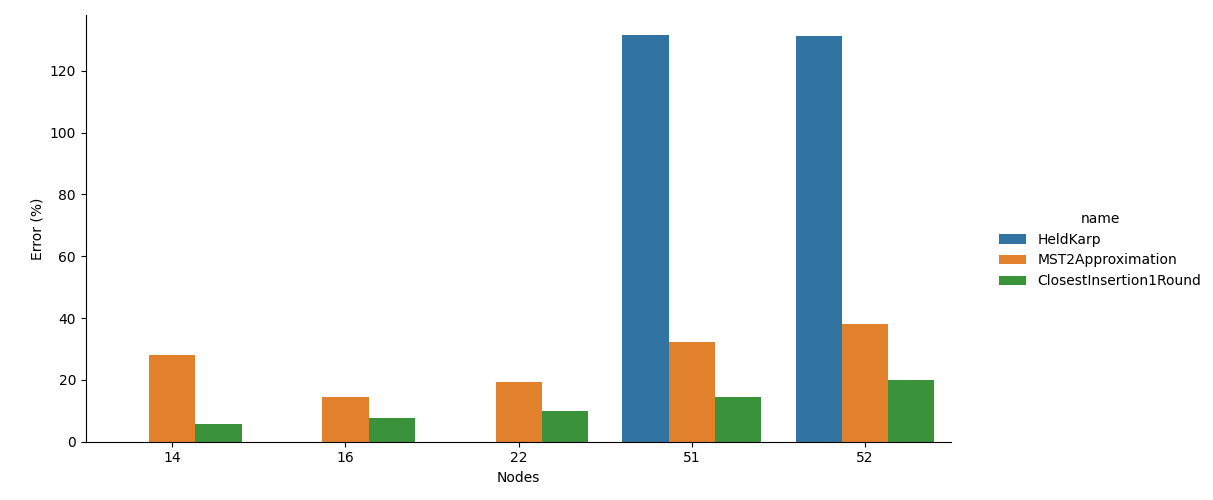
\includegraphics[width=0.9\textwidth]{./images/HeldKarp_vs_MST2Approximation_vs_ClosestInsertion1Round__approximation_error__limited_to_52_nodes_.png}

    \caption{Confronto dell'errore introdotto da Held \& Karp, MST 2-approssimato e Closest Insertion rispetto al numero di nodi (da 14 a 52)}
    \label{fig:heldkarp-mst2approx-closestinsertion-accuracy-error-52-nodes}
\end{figure}

\begin{figure}[H]
    \centering

    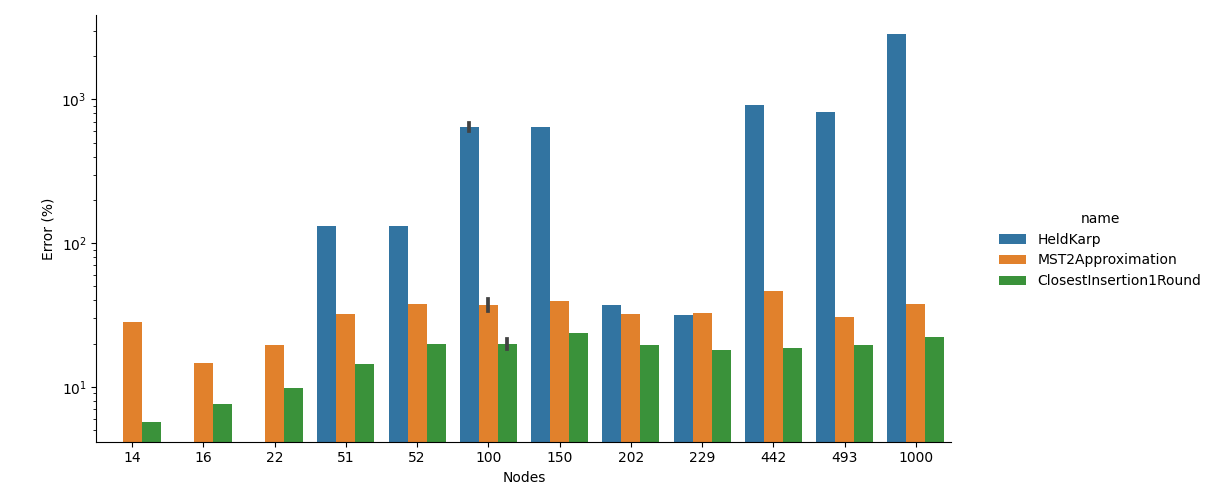
\includegraphics[width=0.9\textwidth]{./images/HeldKarp_vs_MST2Approximation_vs_ClosestInsertion1Round__approximation_error__y_log_scaled_.png}

    \caption{Confronto dell'errore introdotto da Held \& Karp, MST 2-approssimato e Closest Insertion rispetto al numero di nodi (errore in scala logaritmica)}
    \label{fig:heldkarp-mst2approx-closestinsertion-accuracy-error}
\end{figure}

\noindent Il grafico che mostra i tempi di esecuzione per tutti e tre
gli algoritmi non è stato riportato, in quanto ritenuto veramente poco
informativo: Held \& Karp va in timeout dopo i ventidue nodi (con il
timeout fissato a due minuti), mentre il meno efficiente degli altri
termina in poco più di un secondo sul grafo più grande. Abbiamo
inserito quindi il grafico
\ref{fig:mst2approx-closestinsertion-runtime} per confrontare il
runtime di MST 2-approssimato e Closest Insertion, che conferma
l'efficienza in termini di tempi di esecuzione del primo.

\begin{figure}[H]
    \centering

    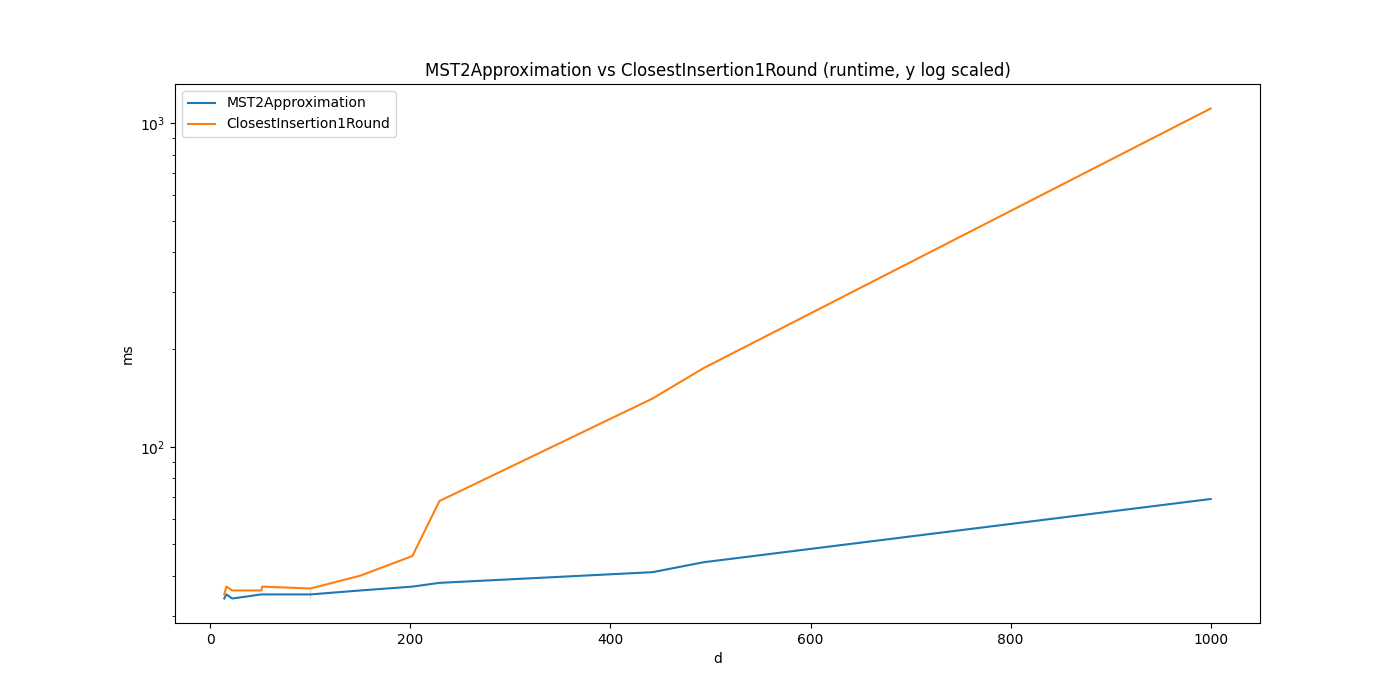
\includegraphics[width=0.9\textwidth]{./images/MST2Approximation_vs_ClosestInsertion1Round__runtime__y_log_scaled_.png}

    \caption{Confronto dei tempi di esecuzione per MST2Approximation e ClosestInsertion rispetto al numero di nodi (runtime in scala logaritmica)}
    \label{fig:mst2approx-closestinsertion-runtime}
\end{figure}

\subsection{Domanda \#2}
\label{sec:question-2}

\begin{displayquote}
Commentate i risultati che avete ottenuto: come si comportano gli
algoritmi rispetti alle varie istanze? C'è un algoritmo che riesce
sempre a fare meglio degli altri rispetto all'errore di
approssimazione? Quale dei tre algoritmi che avete implementato è
più efficiente?
\end{displayquote}

\noindent Gli algoritmi che abbiamo deciso di analizzare, come scritto
nella sezione \ref{sec:question-1}, sono Held \& Karp, MST 2-approssimato e
Closest Insertion. I dati riportati dalle tabelle e dai grafici sono di
facile lettura. Di seguito sono riportate alcune osservazioni sui
risultati ottenuti. \\

\noindent L'algoritmo che riesce
sempre a fare meglio degli altri rispetto all'errore di
approssimazione è Closest Insertion. L'algoritmo riesce a fare sempre meglio di Held Karp (con timeout) e di
MST 2-approssimato. L'errore introdotto è in media relativamente basso:
anche per input piuttosto grandi esso rimane costante intorno al 20\%
circa rispetto alla soluzione ottima. Per grafi di bassa dimensione (sotto ai 100 nodi) i tempi sono comparabili a quelli di MST 2-approssimato, per poi crescere in maniera quadratica, come ci attendevamo data la complessità temporale dell'algoritmo. \\

\noindent L'algoritmo più efficiente dal punto di vista del tempo di
esecuzione è invece MST 2-approssimato.  Quest'ultimo introduce un
errore di approssimazione non trascurabile anche su taglie piccole
dell'input, ma compensa ciò con il tempo di esecuzione dell'algoritmo
che, per dare un'idea, è inferiore ai 70 millisecondi sul grafo più
grande testato. L'approssimazione introdotta, a parte l'oscillazione
iniziale, rimane pressoché costante, intorno al 30/40\% di errore
rispetto alla soluzione ottima. Soprattutto nel caso di grafi di grossa taglia, quest'approssimazione può essere considerata soddisfacente. \\

\noindent Closest Insertion, anche se non è l'algoritmo più veloce
dei tre, ha buoni tempi di esecuzione, e nonostante sia di 2-approssimazione come l'algoritmo che usa il Minimum Spanning Tree, sembra avere un errore medio minore in pratica.

\paragraph{Osservazioni}

\begin{itemize}
    \item L'algoritmo di Held \& Karp, anche per taglie piccole dell'input
      va in timeout e sopra i 22 nodi inizia a restituire delle
      soluzioni parziali che si discostano molto dalla soluzione
      esatta. Questo fenomeno aumenta di molto soprattutto su taglie
      grosse dell'input, anche se è possibile notare un'inversione di
      tendenza per le istanze \emph{gr202} e \emph{gr229}, dove
      l'errore introdotto da Held \& Karp è simile a quello di
      MST2Approximation. È possibile ipotizzare che questo fenomeno
      si verifichi per via della distribuzione dei nodi e quindi del
      valore che gli archi assumono, ma rimane un evento limitato, tra
      l'altro a due istanze la cui sorgente di dati è la stessa. \\

    \item Nella sezione \ref{cap:extensions-and-originalities} abbiamo
      descritto altri algoritmi per la risoluzione di TSP che abbiamo
      deciso di approfondire. In particolare, abbiamo verificato
      empiricamente che l'euristica costruttiva Farthest Insertion
      funziona meglio di Closes tInsertion, e anzi, riesce a fare
      meglio per ogni istanza, con un'errore di approssimazione che
      rimane veramente basso. Per ulteriori dettagli si veda la
      sezione \ref{sec:farthest-insertion}. \\
\end{itemize}

\subsection{Altre misurazioni}

\begin{table}[h!]
    \centering

    \begin{tabular}{lrrrr}
    \toprule
    \multicolumn{5}{c}{Farthest Insertion (standard)} \\
    \hline
     Istanza       &   Esatta &        Soluzione &   Tempo (ms) &   Errore (\%) \\
    \hline
 burma14.tsp   &     3323 &   3323           &           35 &         0    \\
 ulysses16.tsp &     6859 &   6906           &           35 &         0.69 \\
 ulysses22.tsp &     7013 &   7185           &           36 &         2.45 \\
 eil51.tsp     &      426 &    452           &           36 &         6.1  \\
 berlin52.tsp  &     7542 &   8145.5         &           35 &         8    \\
 kroA100.tsp   &    21282 &  22756           &           37 &         6.93 \\
 kroD100.tsp   &    21294 &  22627           &           37 &         6.26 \\
 ch150.tsp     &     6528 &   7097.5         &           41 &         8.72 \\
 gr202.tsp     &    40160 &  43276.5         &           46 &         7.76 \\
 gr229.tsp     &   134602 & 146236           &           69 &         8.64 \\
 pcb442.tsp    &    50778 &  57289.5         &          138 &        12.82 \\
 d493.tsp      &    35002 &  38399.5         &          176 &         9.71 \\
 dsj1000.tsp   & 18659688 &   20632741 &         1114 &        10.57 \\
    \bottomrule
    \end{tabular}

    \caption{Tempo di esecuzione e errore introdotto da Farthest Insertion (standard) rispetto alle istanze.}
    \label{table:farthest-insertion-runtime-accuracy}
\end{table}

\begin{table}[h!]
    \centering

    \begin{tabular}{lrrrr}
    \toprule
    \multicolumn{5}{c}{Farthest Insertion (alternativo)} \\
    \hline
     Istanza       &   Esatta &        Soluzione &   Tempo (ms) &   Errore (\%) \\
    \hline
 burma14.tsp   &     3323 &   3323           &           35 &         0    \\
 ulysses16.tsp &     6859 &   6859           &           35 &         0    \\
 ulysses22.tsp &     7013 &   7013           &           36 &         0    \\
 eil51.tsp     &      426 &    439           &           36 &         3.05 \\
 berlin52.tsp  &     7542 &   8118           &           36 &         7.64 \\
 kroA100.tsp   &    21282 &  23373           &           36 &         9.83 \\
 kroD100.tsp   &    21294 &  22577           &           36 &         6.03 \\
 ch150.tsp     &     6528 &   6864           &           39 &         5.15 \\
 gr202.tsp     &    40160 &  45211           &           45 &        12.58 \\
 gr229.tsp     &   134602 & 148324           &           52 &        10.19 \\
 pcb442.tsp    &    50778 &  56964           &          139 &        12.18 \\
 d493.tsp      &    35002 &  39506           &          173 &        12.87 \\
 dsj1000.tsp   & 18659688 &  20599827.0 &         1110 &        10.4  \\
    \bottomrule
    \end{tabular}

    \caption{Tempo di esecuzione e errore introdotto da Farthest Insertion (alternativo) rispetto alle istanze.}
    \label{table:farthest-insertion-alt-runtime-accuracy}
\end{table}

\begin{table}[h!]
    \centering

    \begin{tabular}{lrrrr}
    \toprule
    \multicolumn{5}{c}{Simulated Annealing} \\
    \hline
     Istanza       &   Esatta &        Soluzione &   Tempo (ms) &   Errore (\%) \\
    \hline
 burma14.tsp   &     3323 &   3854         &           37 &        15.97 \\
 ulysses16.tsp &     6859 &   7580           &           37 &        10.51 \\
 ulysses22.tsp &     7013 &   7802           &           38 &        11.25 \\
 eil51.tsp     &      426 &    518           &           38 &        21.6  \\
 berlin52.tsp  &     7542 &   9412         &           41 &        24.7  \\
 kroA100.tsp   &    21282 &  29467           &           43 &        38.46 \\
 kroD100.tsp   &    21294 &  28883         &           43 &        35.64 \\
 ch150.tsp     &     6528 &   9429         &           47 &        44.43 \\
 gr202.tsp     &    40160 &  54934           &           52 &        36.79 \\
 gr229.tsp     &   134602 & 198875           &           63 &        47.75 \\
 pcb442.tsp    &    50778 &  99430           &           86 &        95.81 \\
 d493.tsp      &    35002 &  61207           &          105 &        74.87 \\
 dsj1000.tsp   & 18659688 &   100466716.0 &          293 &       438.42 \\
    \bottomrule
    \end{tabular}
    \caption{Tempo di esecuzione e errore introdotto da Simulated Annealing rispetto alle istanze.}
    \label{table:simulated-annealing-runtime-accuracy}
\end{table}

Per completezza, riportiamo nelle tabelle \ref{table:farthest-insertion-runtime-accuracy}, \ref{table:farthest-insertion-alt-runtime-accuracy} e \ref{table:simulated-annealing-runtime-accuracy} i tempi e degli errori percentuali relativi agli algoritmi presentati nella sezione \hyperref[cap:extensions-and-originalities]{Estensioni e originalità}. \\

\noindent Si osservi il curioso caso di Simulated Annealing: sembra comportarsi come un algoritmo di 2-approsimazione fino a 493 nodi, per poi esplodere nell'errore nel grafico casuale da 1000 nodi. Possiamo ipotizzare che i parametri usati in Simulated Annealing funzionino bene solo per istanze non troppo grandi. È però anche ragionevole pensare che, se \codeinline{dsj1000} non fosse un grafo costruito artificialmente, forse avremmo avuto un errore di approssimazione migliore.
